\scanpage{108}

\mspage{\handwritten{\unsure{114}}}\handwritten{\unsure{vide|v°}}

\mspage{\handwritten{117}}

Sans parler des \uline{cancéreux} qui font une métastase immédiatement après la vaccination (quand j'étais étudiante, le cancer était une contre-indication de la vaccination, elle ne l'est plus). Un de mes oncles parti en Afrique en pleine santé et réussite professionnelle pour un safari a dû subir toutes les vaccinations d'usage. Il est revenu épuisé et est mort dans l'année, de \deleted{leucémie.}

\deleted{Coïncidence ? Justement ça coïncide et c'est cette coïncidence que la science devrait expliquer.}

\deleted{Voici encore l'exemple de cette petite fille atteinte d'ipsa rythmie, guérie par un traitement cortisoné dans sa première enfance (maladie cérébrale entraînant idiotie et épilepsie). A 9 ans, le pédiatre déclare qu'on peut la vacciner ``puis qu'elle est guérie''. Depuis elle est épileptique. Elle a 16 ans.}

Coïncidence ? L'ennui c'est que cette coïncidence est fréquente dans l'épilepsie. J'en traite plusieurs cas qui se sont manifestés ``à l'âge des vaccinations''.

Et \unsure{cėtte|cètte|cette} petite fille vue à 6 mois se développant parfaitement bien cependant, qui débute une maladie de Little à 11 mois, aussitôt après la 1ère vaccination. Elle n'aura pas le tétanos, mais elle est paraplégique.

Coïncidence ? Justement ça coïncide étrangement et tant que l'on aura pas prouvé qu'il n'y a aucun lien entre la vaccination et la maladie qui ``coïncide'' comment obliger les parents à prendre ce risque.

Le 15 mai 1986, j'ai reçu une jeune femme pour troubles dépressifs, suite à la mort par encéphalite, 5 jours après une vaccination par le D.T.COQ, de son nourrisson de 4 mois. Cette vaccination ne faisait pas partie du lot retiré pour 48H. et l'accident n'a pas été communiqué à la presse.

\deleted{On ne convaincra jamais la maman qu'il ne s'agit que d'une coïncidence.}

\deleted{Est-ce une coïncidence aussi, ce que déclare le Dr.SARTORIUS de l'O.M.S. : ``On protège les enfants contre les maladies aigües, mais le nombre de maladies chroniques spécifiques s'accroit plus vite qu' l'ensemble de la popula\uuline{ti}on''.}

\deleted{Na-t-on pas le droit de choisir pour soi ou ses enfants entre le risque de maladie aigüe et le risque de maladie chronique ?}

\deleted{Ce même Dr. SARTORIUS nous dit encore : ``Pour les individus ayant vécu jusqu'à 65 ans, l'espérance de vie est de 75 ans dans les pays non médicalisés (le Nigéria par exemple) \deleted{comme} dans les pays d'Europe''.}

\deleted{Devons-nous donc être tellement fiers et sûrs de nos techniques au point de les imposer par l'obligation ?}

\deleted{Que l'on ne s'imagine pas que nous réclamons d'interdire les vaccinations ; les gens ont le droit de se protéger et protéger leurs enfants, ou leur chep}tel,des maladies aigües, par les vaccinations.

Ce que nous réclamons, et personnellement je le réclame à plusieurs titres :

- comme médecin homœopathe ayant à sa disposition une médecine prophylactique.

- comme française ayant hérité des valeurs de 1789.

- comme membre de l'A.C.A.T. luttant pour les droits de l'homme.

Ce que nous réclamons est très simple :

Que l'état laisse aux gens la liberté de choisir leur prophylaxie, même au risque de se tromper : ``errare humanum est'' et c'est sa grandeur. Et que ceux qui ont choisi la meilleure médecine soient récompensés par la meilleure santé qui leur servira de preuve.

\ldots/\ldots

\deleted{Voilà les faits que j'ai voulu résumer pour éclairer la Cour, sans l'ennuyer par de longs discours, au sujet du difficile problème que pose le procès de Monsieur COULARDEAU.}

\deleted{Ces faits parlent d'eux mêmes pour montrer que la médecine qu'a choisie Monsieur COULARDEAU pour garantir la santé de son troupeau vaut bien la facile vaccination et qu'en se donnant le mal de traiter ses bêtes par une thérapie individualisée il leur confère un degré de santé supérieure à celle qui est simplement requise par la loi au moyen des vaccinations. Je répéterai donc ce qu'ont signé mes 26 confrères homœopathes dans leur lettre à Monsieur le Préfet de la Haute-Loire : Monsieur COULARDEAU a satisfait à l'esprit de la loi plus que ceux qui satisfont à la lettre, et en attendant que soit réformé la lettre au nom de l'esprit qui l'a inspirée, nous espérons que Monsieur COULARDEAU sera jugé en fonction de cet esprit.}

\handwritten{\unsure{S Fayeton|A Fayeton|S. Fayeton}.}\\

% printed form
Docteur Simone FAYETON\\
01 - Généraliste \qquad Conventionné Hon. Lib.\\
Le Clos de Corsac\\
43700 BRIVES CHARENSAC\\
43 1 00308 6

\figure{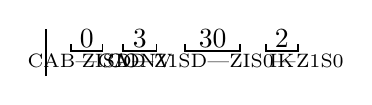
\begin{tikzpicture}[x=.66cm,y=.66cm,every node/.style={inner sep=0pt}]
\draw[line width=.8pt] (0,-.49)--(0,.42); \node at (.78,.24) {0}; \node at (1.80,.24) {3}; \node at (3.20,.24) {30}; \node at (4.53,.24) {2}; \draw[line width=.65pt] (.48,.12)--(.48,0)--(1.08,0)--(1.08,.12); \draw[line width=.65pt] (1.48,.12)--(1.48,0)--(2.12,0)--(2.12,.12); \draw[line width=.65pt] (2.67,.12)--(2.67,0)--(3.73,0)--(3.73,.12); \draw[line width=.65pt] (4.22,.12)--(4.22,0)--(4.84,0)--(4.84,.12); \node[font=\scriptsize] at (.78,-.20) {\unsure{CAB|CAD}}; \node[font=\scriptsize] at (1.80,-.20) {CONV}; \node[font=\scriptsize] at (3.20,-.20) {\unsure{ZISD|Z1SD|ZIS0|Z1S0}}; \node[font=\scriptsize] at (4.53,-.20) {IK};
\end{tikzpicture}}

% archive sheet number: 108
